\documentclass[11pt]{article}

\usepackage[utf8]{inputenc}
\usepackage{listings}
\usepackage{color}
\usepackage{graphicx}
\usepackage{url} % for references, which require url's
% \usepackage[ngerman]{babel}
\setlength{\textwidth}{5.5in}

\title{Corba Übung}
\author{Nikolaus Schrack, Gary Ye (4BHIT)}
\date{\today{}, Wien}
\begin{document}

\maketitle
\newpage % Borko Style 
\tableofcontents
\newpage

\lstset{basicstyle=\ttfamily\small,
        keywordstyle=,
        commentstyle=\itshape,
        numbers=left,                   % where to put the line-numbers
        stepnumber=1,
        breaklines=true,					% line wrapping on
        numberstyle=\tiny,
        showstringspaces=false,
        abovecaptionskip=0pt,
        belowcaptionskip=0pt,
        xleftmargin=\parindent,
        fontadjust}

\section{Aufgabenstellung}
Verwenden Sie das Paket ORBacus oder omniORB bzw. JacORB um Java und C++ ORB-Implementationen zum Laufen zu bringen.

Passen Sie eines der Demoprogramme so an, dass Sie einen Namingservice verwenden, welches ein Objekt anbietet, das von jeweils einer anderen Sprache (Java/C++) verteilt angesprochen wird. Beachten Sie dabei, dass eine IDL-Implementierung vorhanden ist um die unterschiedlichen Sprachen abgleichen zu können.

Vorschlag: Verwenden Sie für die Implementierungsumgebung eine Linux-Distribution, da eine optionale Kompilierung einfacher zu konfigurieren ist.

\subsection{Resources}

\begin{itemize}
\item http://omniorb.sourceforge.net/
\item http://www.microfocus.com/products/corba/orbacus/
\item http://www.jacorb.org/
\item http://omniorb.sourceforge.net/omni41/omniORB.pdf
\item http://www.ing.iac.es/~docs/external/corba/book.pdf
\end{itemize}

\section{Aufwandsschätzung}
\subsection{Geschätzter Aufwand}

\begin{center}
  \begin{tabular}{| l | l | l |}
    \hline
    Task & Schrack & Ye \\ \hline

    Dokumentierung des C++ Servers   & 3h & \\ \hline
    Dokumentierung des Java Clients  & & 6h \\ \hline
    Implementierung des Java Clients & & 4h \\ \hline \hline
    Gesamt & 3h & 10h \\ \hline
  \end{tabular}
\end{center}

\subsection{Tatsächlicher Aufwand}
\begin{center}
  \begin{tabular}{| l | l | l |}
    \hline
    Task & Schrack & Ye \\ \hline
    Dokumentation Allgemein          & 1h & 5h \\ \hline
    Dokumentierung des C++ Servers   & 2h & 0.5h\\ \hline
    Dokumentierung des Java Clients  & & 2h \\ \hline
    Implementierung des Java Clients & & 2h \\ \hline \hline
    Gesamt & 3h & 9.5h \\ \hline
  \end{tabular}
\end{center}

Weil wenig Erfahrung in dem Gebiet besteht, wurde eine sehr hohe Aufwandszeit geschätzt. Die Zeit wurde hauptsächlich mit dem Lesen der beiliegenden Dokumentationen \cite{omniorbuserguide} verbracht, damit das Implementieren ohne Zweifeln ausgeführt werden konnte.

\section{Arbeitsaufteilung und Designüberlegung}
Da beide Teammitglieder Corba-Neulinge sind, wurde aus Erfahrung beschlossen, dass das Lesen der Dokumentationen der beste Start in eine neue Übung bzw. Aufgabe ist. Nachher sind die neue Technologien und der Quellcode, der beiliegenden Beispiele, einigermaßen klarer geworden. Im omniORB-Verzeichnis gibt es ein ``echo-example'', das eine in C++ implementierte Version von Server und Client, die den NamingService verwenden, enthält. Danach wurde ausgemacht, dass Gary Ye die Java Client Version schreibt und seine Vorgänge niederschreibt, und dass Nikolaus Schrack den größten Teil des C++ Source Codes dokumentiert. 

\section{Installation}

\subsection{OmniORB}

Die folgende Packages werden für die Installation von OmniORB benötigt: omniorb omniorb-doc omniorb-idl omniorb-nameserver python2.7-dev. Diese sollten entsprechend mit apt-get installiert werden und danach ladet man die Installationsdateien von der offiziellen OmniORB Seite \cite{omniorbpage} runter (es wurde für die Übung omniORB-4.1.7 benutzt). Anschließend wechselt man in den Omniorb Directory und führt die folgende Befehle, die auch im Readme erwähnt sind, aus.

\begin{lstlisting}
mkdir build
cd build
../configure
make
make install
\end{lstlisting}

Man kann auch den Installationsort ändern, indem man einen Wert für --prefix angibt. Sollte man keinen angeben, so werden sie per Default im /usr/local Verzeichnis installiert.

\begin{lstlisting}
../configure --prefix=/home/gary/omni_inst
\end{lstlisting}

\subsection{JacORB}

Es wird Apache Ant benötigt, um die Sourcefiles von JacORB zu kompilieren.

\begin{lstlisting}
wget http://www.jacorb.org/releases/3.2/jacorb-3.2-source.zip
unzip jacorb-3.2-source.zip
cd jacorb-3.2
ant all
\end{lstlisting}

Wenn eine neuere Version als 3.2 erwünscht ist, dann sollte man sie von der offiziellen Website runterladen!\cite{jacorbpage}

\section{Implementierung}

\subsection{IDL File}

IDL (Interface Definition Language) ist eine deskriptive Sprache zum Beschreiben der Interfaces in einem Softwareprogramm. Das Beschreiben geschieht Programmiersprache-unabhängig, damit Softwarekomponenten, die in verschiedenen Programmiersprachen geschrieben wurden (wie z.B. C++, Java, Python), miteinander kommunizieren können. Man kann das IDL File mit Hilfe eines IDL Compilers zu einem sprachspezfischen Quellcode kompillieren (z.B. Stubs, Skeletons, etc.). 

Der folgende Code ist von das am ``Echo'' Inteface angepasste IDL File(echo.idl). Anzumerken ist, dass es einen Modul namens ``schrackye'' existiert. Module sind ähnlich wie Packages von Java oder Namespaces von C++. 

\lstset{language=IDL}  

\begin{lstlisting}
#ifndef __ECHO_IDL__
#define __ECHO_IDL__
module schrackye {
        interface Echo {
                string echoString(in string mesg);
        };
};
#endif // __ECHO_IDL__         

\end{lstlisting}

\begin{description}
\item[Line 1-2, 8] \hfill \\
\#ifndef \_\_ECHO\_IDL sind wie man von C kennt Header Guards, die vor Doppeldeklarationen schützen sollen. 
\item[Line 3] \hfill \\
Man definiert Module wie Namespaces in C++. Man sollte beachten, dass ein Semikolon ``;'' hinter der geschlossenen geschwungenen Klammer ``\}'' gehört.
\item[Line 4] \hfill \\
Die Deklaration von Interfaces kennt man von Java; auch hier muss man am Ende ein Semikolon schreiben.
\item[Line 5] \hfill \\
Die Methode echoString erwartet einen String und gibt auch ein Objekt vom Typ String zurück. Anzumerken ist, dass hier ein ``in'' in der Parameterliste steht. Die Bedeutungen von ``in'', ``out'' und ``inout'' stehen im folgenden Absatz.

The parameters of an operation have a specified direction, which can be in (meaning that the parameter is passed from the client to the server), out (the parameter is passed from the server back to the client) or inout (the parameter is passed in both directions). \footnote{Quelle: http://stackoverflow.com/questions/6264424/corba-idl-in-out-and-inout}
\end{description}
Um das IDL File in Java zu kompilieren benutzt man das von JacORB mitgelieferten Compiler namens idlj:
\lstset{language=bash}
\begin{lstlisting}
idlj echo.idl
\end{lstlisting}
Oder für C++ das von omniORB mitgeliferten Compiler omniidl:
\begin{lstlisting}
omniidl echo.idl
\end{lstlisting}

\subsection{C++ Server}

Der größte Teil vom Code wurde vom Echo Example entnommen. Es werden die essenziellen Teile des Codes beschrieben. 

In dem folgenden Codesnippet wird das Echo Interface implementiert.

\begin{lstlisting}
class Echo_i : public POA_schrackye::Echo
{
public:
  inline Echo_i() {}
  virtual ~Echo_i() {}
  virtual char* echoString(const char* mesg);
};


char* Echo_i::echoString(const char* mesg)
{
  return CORBA::string_dup(mesg);
}
\end{lstlisting}

\begin{description}

\item[Line 10-13] \hfill \\
Die Implementierung der Methode echoString, wo der gegebene String auf die Corba-Art dupliziert wird und anschließend zurückgegeben wird.

\end{description}

Der folgende Code ist ein Teil von der Main Funktion.

\begin{lstlisting}
CORBA::ORB_var orb = CORBA::ORB_init(argc, argv);

CORBA::Object_var obj = orb->resolve_initial_references("RootPOA");
PortableServer::POA_var poa = PortableServer::POA::_narrow(obj);

Echo_i* myecho = new Echo_i();

PortableServer::ObjectId_var myechoid = poa->activate_object(myecho);

obj = myecho->_this();

CORBA::String_var x;
x = orb->object_to_string(obj);
cout << x << endl;

if( !bindObjectToName(orb, obj) )
  return 1;

myecho->_remove_ref();

PortableServer::POAManager_var pman = poa->the_POAManager();
pman->activate();

orb->run();
\end{lstlisting}

\begin{description}

\item[Line 1] \hfill \\
Hier wird der ORB mit den Kommandozeilenargumenten initialisiert.

\item[Line 3-4] \hfill \\
Der Server wird für die Client sichtbar gemacht. Dies wird mit der Registrierung bei dem Portable Server Adapter (in unserem Fall der \textit{Root POA}) durchgeführt.

\item[Line 6] \hfill \\
Eine neue Instanz von Echo wird erstellt.

\item[Line 8] \hfill \\
Das Objekt wird vom POA aktiviert und gibt eine Objekt-Id zurück.

\item[Line 10] \hfill \\
Die Objekt Referenz von myecho wird erlangt und in obj abgespeichert.

\item[Line 12-14] \hfill \\
Eine Corba String Variable x wird initialisiert und ausgegeben. 

\item[Line 16-17] \hfill \\
In der if-Abfrage wird geprüft ob die Bindung vom Naming Server\footnote{Siehe Subsektion NamingService} gelingt.

\item[Line 19] \hfill \\
Die Referenz von myecho wird gelöscht, jedoch exisitiert noch eine Referenz auf das Objekt noch in POA.

\item[Line 21-22] \hfill \\
Der Portable Object Adapter Manager wird aktiviert, da POAs anfangs in einem "holding" State sind (d.h. einkommende Anfragen werden ignoriert).

\item[Line 24] \hfill \\
Der Object Request Broker (ORB) wird gestartet.

\end{description}

\subsubsection{NamingService}
Der NameService bietet eine komfortabelere Alternative zu IOR Strings an. Man muss nur die richtige Sequenz von \textit{NameComponents} angeben, um das gewünschte Objekt zu bekommen. Der Name eines Objektes kann man mit einem String beschreiben, wobei man NameComponents mit Slashes "/" trennt. Außerdem hat jedes NameComponent eine Form von \textit{"id.kind"}. Beispiel wäre ``test.my\_context/Echo.Object'', das auch im Laufe der Übung für das Echo Objekt verwendet wurde.
\begin{itemize}
\item Der NameService von omniORB (C++) heißt ``omniNames''.
\item Der NameService von JacORB heißt ``ns''.
\end{itemize}
\subsection{Java Client}

Der folgende Java Code führt einen Remote Procedure Call (RPC) aus, um eine Nachricht, die man an den Server übergibt, von ihm wieder zurückbekommt (also im Prinzip der Aufruf der Methode echoString).

\begin{lstlisting}
package schrackye;

import java.util.Properties;

import org.omg.CosNaming.*;
import org.omg.CosNaming.NamingContextPackage.InvalidName;

public class Client {
    public static void main(String[] args){
	Echo echo;
	try{
	    org.omg.CORBA.ORB orb = org.omg.CORBA.ORB.init(args, null);

	    org.omg.CORBA.Object o = orb.resolve_initial_references("NameService");
	    NamingContextExt rootContext = NamingContextExtHelper.narrow( o );
			
	    NameComponent[] name = new NameComponent[2];
	    name[0] = new NameComponent("test","my_context");
	    name[1] = new NameComponent("Echo", "Object");
		
	    echo = EchoHelper.narrow(rootContext.resolve(name));
	    System.out.println("Server says : " + echo.echoString("Juhu funktioniert!"));
	} catch(InvalidName e){
	    System.err.println("InvalidNameException occured : " + e.getMessage());
	} catch(Exception e){
	    System.err.println("Unknown exception occured : " + e.getMessage());
	    e.printStackTrace();
	}
    }
}
\end{lstlisting}

\begin{description}
\item[Line 12] \hfill \\
Hier initialisiert man den ORB. Man übergibt ih die Programmargumente ``args'' von der Kommandozeile und er bearbeitet alle, die den Präfix ``-ORB'' besitzen. Die Kommandoargumente ist eine Alternative zu dem Property File.

\item[Line 14-15] \hfill \\
Hier erhält man den RootContext des angegebenen Namingservices. 

\item[Line 17-19] \hfill \\
Hier gibt man den Path zu dem Echo Objekt, das man anfragt, an. Ein NamingContext löst nämlich nur Arrays von NameComponents auf. 

\item[Line 21] \hfill \\
Hier wird der Name, den wir angegeben haben, aufgelöst. Da die Methode``resolve()'' ein Objekt vom Typ org.omg.CORBA.Object zurückgibt, muss man mit Hilfe von dem entsprechenden Helper, die Rückgabe in den Ursprungstyp zurückformen lassen (``narrow'').

\item[Line 22] \hfill \\
Die Methode wird mit Hilfe von einem RPC aufgerufen und das Ergebnis lässt sich dann im Output sehen.

\end{description}

\section{Ausführung}
\subsection{C++ Server}
\subsubsection{Naming Server}
Falls der NamingServer namens omniNames nicht gestartet ist, so muss man ihn manuell starten.
\begin{lstlisting}
omniNames -start
\end{lstlisting}

\subsubsection{Makefile Anpassung}
Zuerst muss man ein wenig das Makefile am eigenen System anpassen. Man muss nur den Installationsort von OmniORB, den man bei --prefix geschrieben hat, angeben.
\begin{lstlisting}
OMNI_HOME     = /usr/local
\end{lstlisting}
\subsubsection{Server Starten}
Schlussendlich den Server starten mit:
\begin{lstlisting}
./server
\end{lstlisting}

\subsection{Java Client}
\subsubsection{Corbaloc}
Mit dem Corbaloc\footnote{(für mehr Infos\cite{book1})} definiert man die Addresse, Portnummer und den Servicename an. In diesem Fall wird beim Aufrufen des Java Clients die Informationen vom NameService übergeben.

Wenn der NameService am Server mit der IP Addresse 192.168.163.129 und der Portnummer 2809 ist, so ist der entsprechende Corbaloc folgender:
\begin{lstlisting}
corbaloc::192.168.163.129:2809/NameService
\end{lstlisting}

\subsection{Ausführung}
Den folgenden Befehl muss man ausführen, um einen Server (mit der IP Addresse 192.168.163.129 Portnummer 2809) anzusprechen. Danach sollte man einen entsprechende Ausgabe bekommen (unter der Vorraussetzung, dass der Server zuerst gestartet wurde und auch von außen ansprechbar ist).

\begin{lstlisting}
java schrackye.Client -ORBInitRef NameService=corbaloc::192.168.163.129:2809/NameService
\end{lstlisting}

\section{Aufgetretene Probleme}
Die meisten Probleme sind nur bei der Erstellung der Makefiles geschehen.
\subsection{Ant File - Args}
Wenn man die folgende Zeile im Ant Buildfile schreibt, so wird dem Programm nur \textit{ein} Argument geben (anstatt erwartete zwei).
\begin{lstlisting}
<arg value=''-ORBInitialPort 2809'' />
\end{lstlisting}

Daher muss man dieses Argument in zwei Ant-Args unterteilen.
\begin{lstlisting}
<arg value=''-ORBInitialPort'' />
<arg value=''2809'' />
\end{lstlisting}


\section{Testbericht}
\subsection{Lokales Testing}

Anfangs wurde nur lokal getestet, d.h. Server und Client sind beide auf der selben Maschine gewesen. Er ist wie auf dem Bild zu sehen, erfolgreich abgelaufen. Das linke Terminal ist eine Debian VirtualMachine (mit SSH verbunden), während auf der rechten Seite eine Ubuntu Maschine läuft.

\begin{center}
  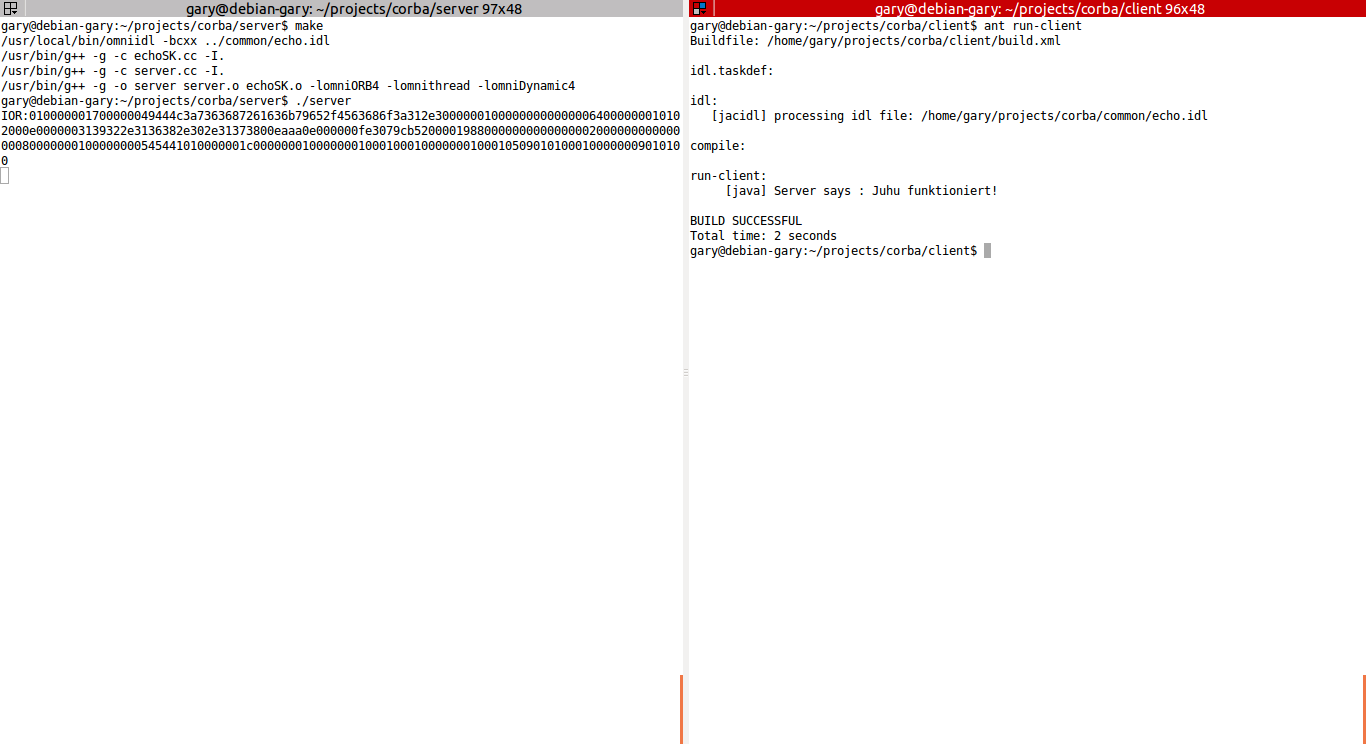
\includegraphics[width=\textwidth, height=1.5in]{test_local}
\end{center}

\subsection{Testing über das Netzwerk}
Noch ein Bild von dem Testen über das Netzwerk, das erfolgreich abgelaufen ist.

\begin{center}
  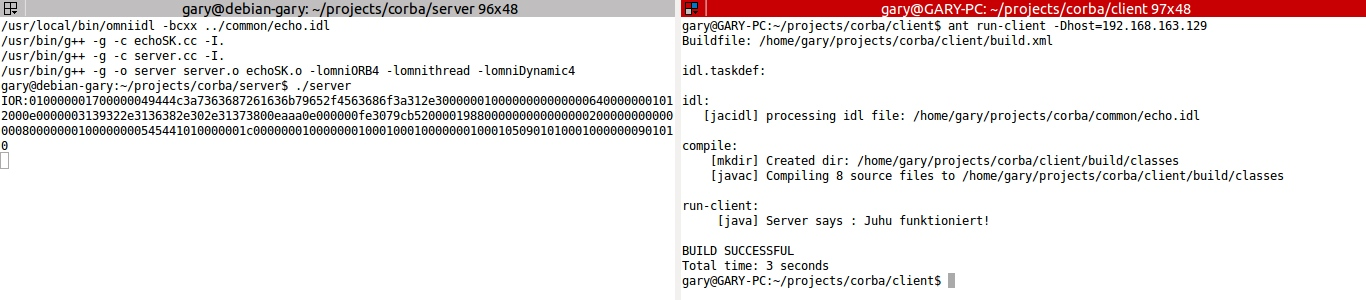
\includegraphics[width=\textwidth, height=1.5in]{test_network}
\end{center}

\section{Siege und Niederlagen}
\subsection{Siege}
\begin{itemize}
\item Der Java Client wurde erfolgreich an dem Echo Example angepasst.
\item Es wurde zum ersten Mal mit \LaTeX  Erfahrung gemacht (erwähnenswert, wenn für die Dokumentation mehr als die Hälfte der Zeit angewendet wurde).
\end{itemize}
\subsection{Niederlagen}
Subjektiv gesehen, gibt es keine Niederlagen.

\bibliography{references}{}
\bibliographystyle{plain}

\end{document}
